\documentclass[11pt]{article}
\usepackage{tikz}
\usepackage{amsmath,graphicx}
\begin{document}
\title{Conservative Overset for Discontinuous Galerkin Methods}
\author{Steve Tran}
\maketitle

\section{Discontinuous Galerkin Formulation}

The problem of interest is the 1D advection equation, shown below in its strong form. 

\begin{equation} 
  u_{,t} + a u_{,x} = 0
  \label{eq:strong}
\end{equation}

\noindent where $u$ is the unknown, $a$ is the convection speed, $x$ is space, and $t$ is time. 
Note that Einsteinian index notation is used. 
Following the traditional finite element formulation, Equation \eqref{eq:strong}
is multiplied by an arbitrary weighting function, $w$, and then is integrated over the domain. 
Using integration by parts, we arrive at  \eqref{eq:weak1}. 

\begin{equation}
\int_\Omega \left[ w u_{,t} - a w_{,x} u \right ]d\Omega + a w u |_\Gamma= 0
\label{eq:weak1}
\end{equation}

\noindent where $\Omega$ represents the domain and $\Gamma$ represents the boundaries of 
the domain. Following the finite element method, the domain is split up into a number of
discrete 1D elements, described by Equation \eqref{eq:weak2}. 

\begin{equation}
\int_{\Omega_e} \left[ w u_{,t} - a w_{,x} u \right ]d{\Omega_e} + a w u|_{\Gamma_e}= 0
\label{eq:weak2}
\end{equation}

\noindent Quantities with the subscript $e$ denote elemental quantities. Next the
weighting function and unknown variables are decomposed into the products of
space-dependent shape functions and time-varying coefficients as follows:

\begin{equation}
w(x,t) = \sum_{i=1}^{nshp} N_i(x) \hat{w}(t)
\end{equation}

\begin{equation}
u(x,t) = \sum_{i=1}^{nshp} N_i(x) \hat{u}(t)
\label{eq:shape}
\end{equation}

\noindent where $N(x)$ are the shape functions, nshp is the number of bases on 
any given element, and $\hat{\cdot}$ denotes the variable coefficients. 
The weighting function and the unknown variable are assumed to occupy the same space so the 
same shape functions are used for both $w$ and $u$, although . 
the exact shape functions used are chosen by the user and may vary from code to code.

The above equations can be substituted into Equation \eqref{eq:weak2} and, recognizing that the
weighting functions are arbitrary and their coefficients may be factored out, we arrive at the
following equation. 

\begin{equation}
\int_{\Omega_e} \left[ N_a N_b \hat{u}_{b,t} - a N_{a,x} N_b \hat{u}_b \right ]d{\Omega_e} + a N_a N_b \hat{u_b}|_{\Gamma_e}= 0
\label{eq:weak3}
\end{equation}

Note again that Einstein notation is used so repeated indicies imply a summation. Then
rearranging we arrive at the final equation that the code will solve. 
   
\begin{equation}
\hat{u}_{b,t} \int_{\Omega_e} N_a N_b d{\Omega_e} - \int_{\Omega_e} a N_{a,x} N_b \hat{u}_b d{\Omega_e} + a N_a N_b \hat{u_b}|_{\Gamma_e}= 0
\label{eq:weak4}
\end{equation}

Observe that this represents a system of equations for each element. 
The first term in Equation \eqref{eq:weak4}, called the ``mass matrix'',
is a matrix of size $nshp \times nshp$ whereas the second and third terms, the convective and 
flux terms, respectively, are vectors of length nshp.
 
Using the discontinuous Galerkin (DG) approach, there is no requirement for
the values of $u$ to be continous across elements, as shown in Figure{fig:dg}. 
Thus, special care must be taken with the flux vector, $a N_a N_b u_b |_{\Gamma_e}$,
in order to approximate the inter-element fluxes. In this work, a simple
upwinding approach is used. 

\begin{figure}[h]
\centering
  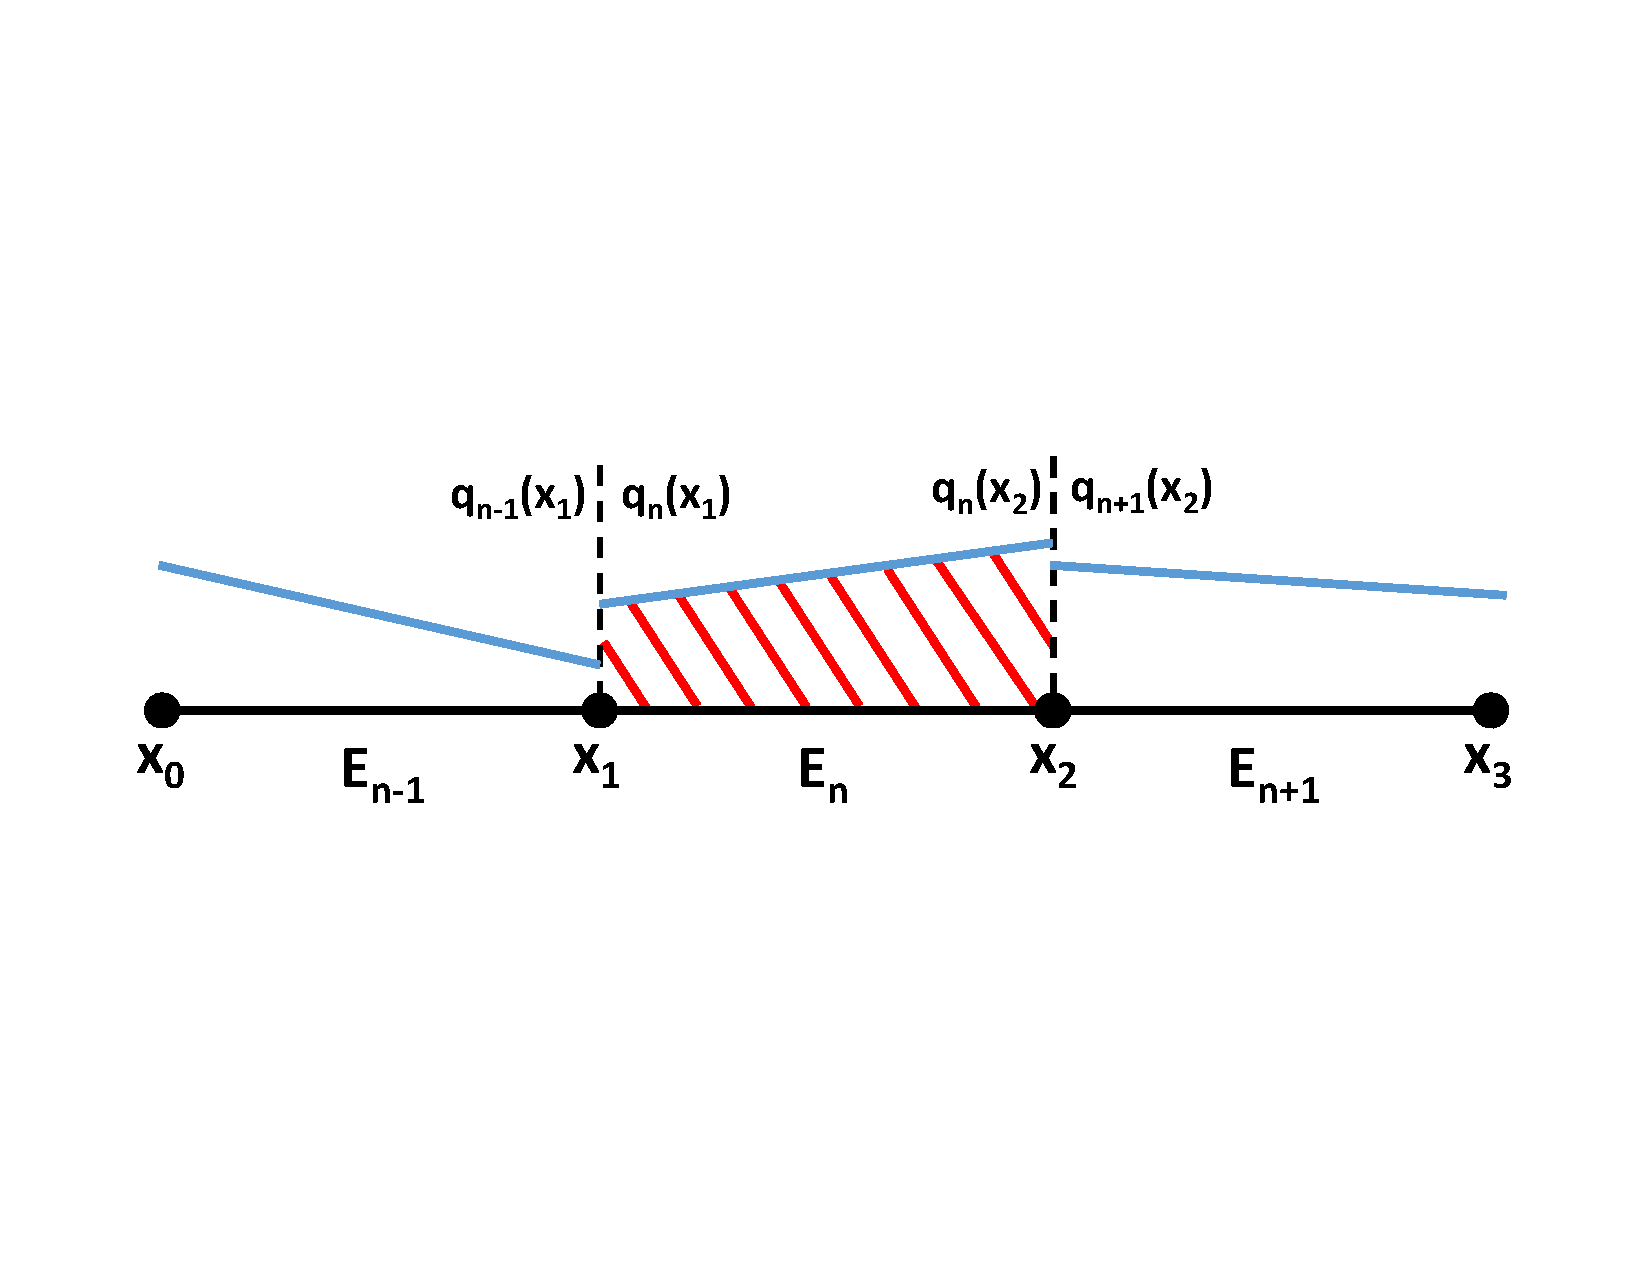
\includegraphics[width=\textwidth,trim={0 8cm 0  7cm},clip]{DGDiagram.pdf}
  \caption{Schematic describing a conventional DG method on a single mesh, with fluxes calculated at the discontinuous boundaries and volume integrals calculated over the element (shown in striped red)}
  \label{fig:dg}
\end{figure}

\begin{equation}
a u|_{\Gamma_e} \approx 0.5( a (u_L + u_R) - |a| (u_R-u_L))
\label{eq:upwind}
\end{equation} 

\noindent where $u_L$ and $u_R$ represent the left and right states of $u$ across
the element boundaries. 

The volume integral terms needed to compute the mass matrix and the convective
terms are found using numerical quadrature. In this case, Gauss-Legendre quadrature
was used. For the time integration, the explicit third order Runge Kutta scheme
was applied.  

\section{Overset Approach}

Two methods are used to handle situations where the problem is solved on two or more
separate but overlapping grids (ie overset meshes). 

\begin{figure}[t]
\centering
  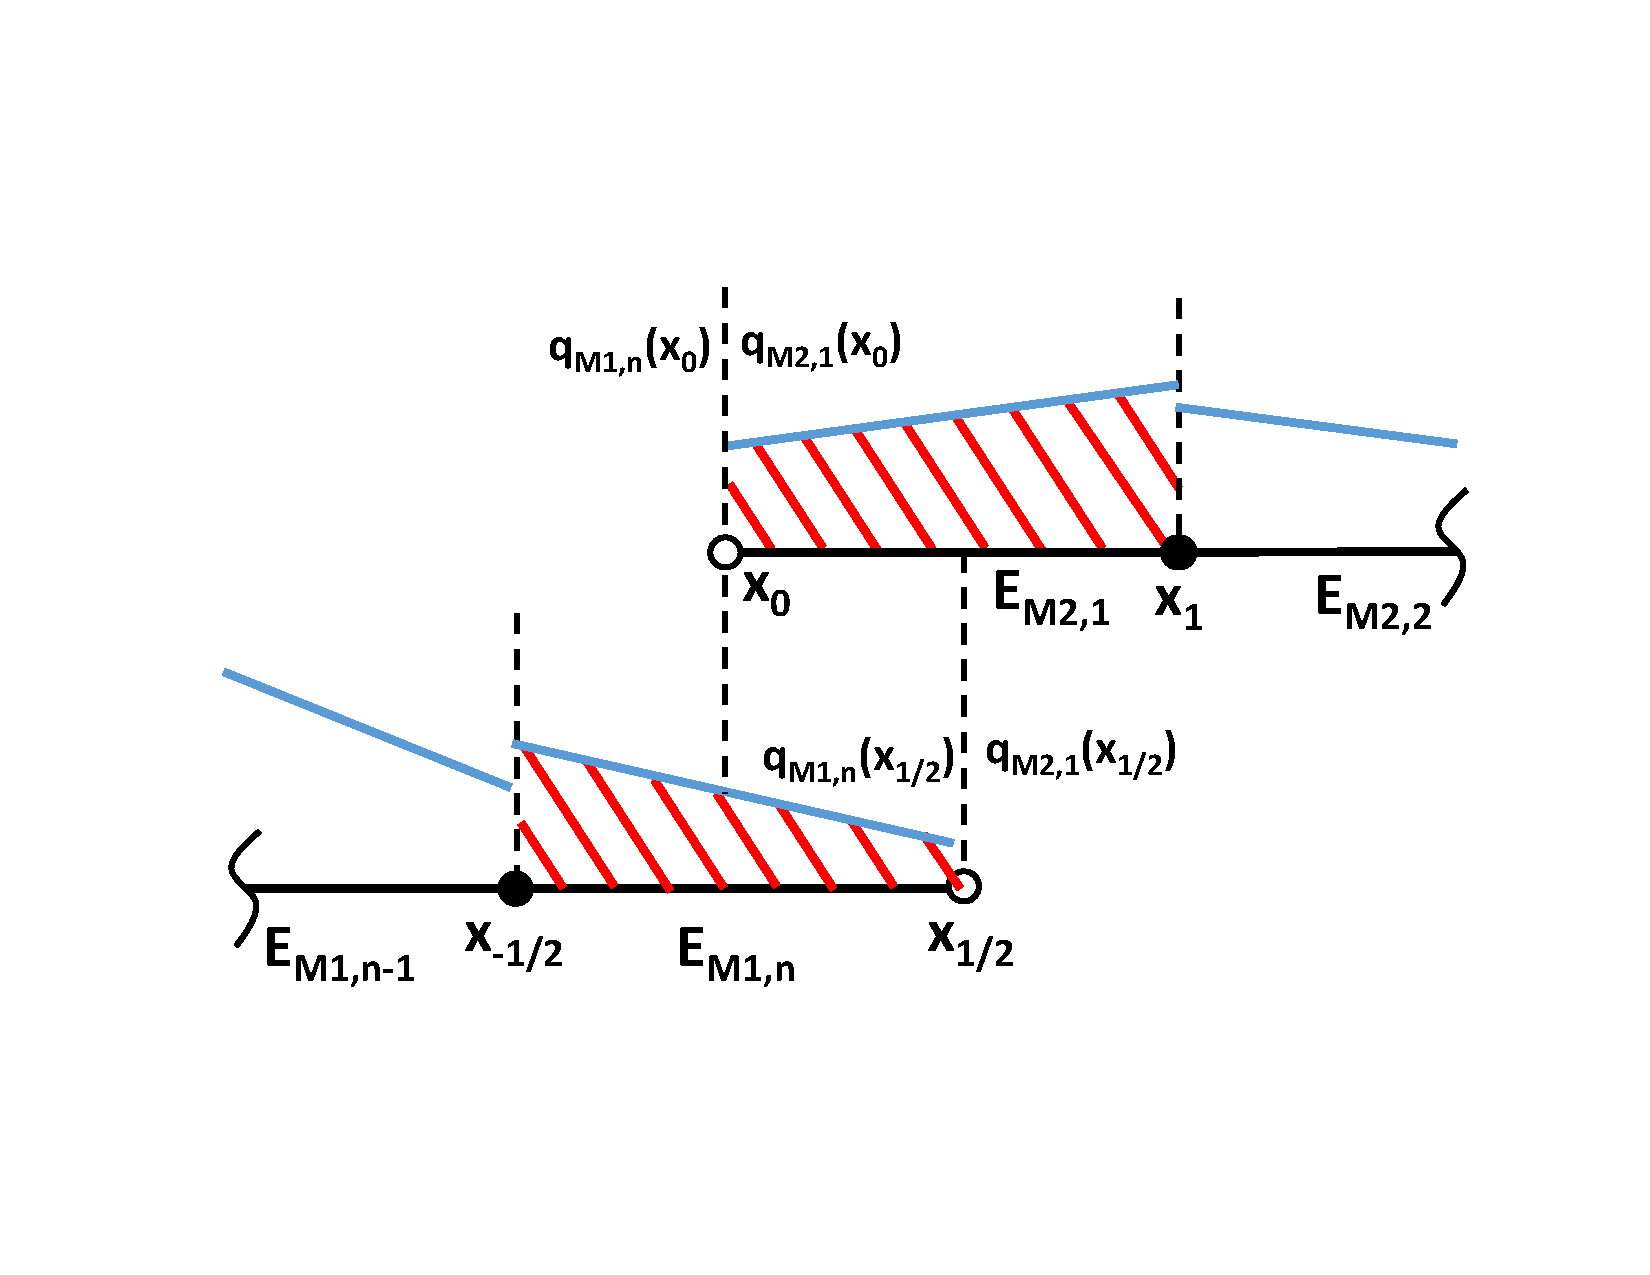
\includegraphics[width=\textwidth,trim={0 4cm 0 4cm},clip]{DGBaseOverset.pdf}
  \caption{Schematic describing the baseline overset DG method with two meshes. Fluxes from neighboring meshes are interpolated at the element endpoints and volume integrals are calculated over the complete elements (shown in striped red)}
  \label{fig:base}
\end{figure}

The first method, called the Baseline Method here, is described visually in Figure \ref{fig:base}. 
Using this method, the fringe elements are handled similarly to the interior elements. The volume
integrals for the mass matrix and convective terms are integrated as normal using the local values 
of $\hat{u}$. For the flux vector, the contribution from the neighboring mesh is interpolated
at the interior of the neighboring meshe's fringe element, and not its end point as is typically done. 
This interpolation is done using the typical finite element approach, shown in Equation 
\eqref{eq:shape}.This method leads to stable and convergent solutions
however conservation error is incurred since the contributions from the overlapping region is counted
twice, once on each mesh.

\begin{figure}[h]
\centering
  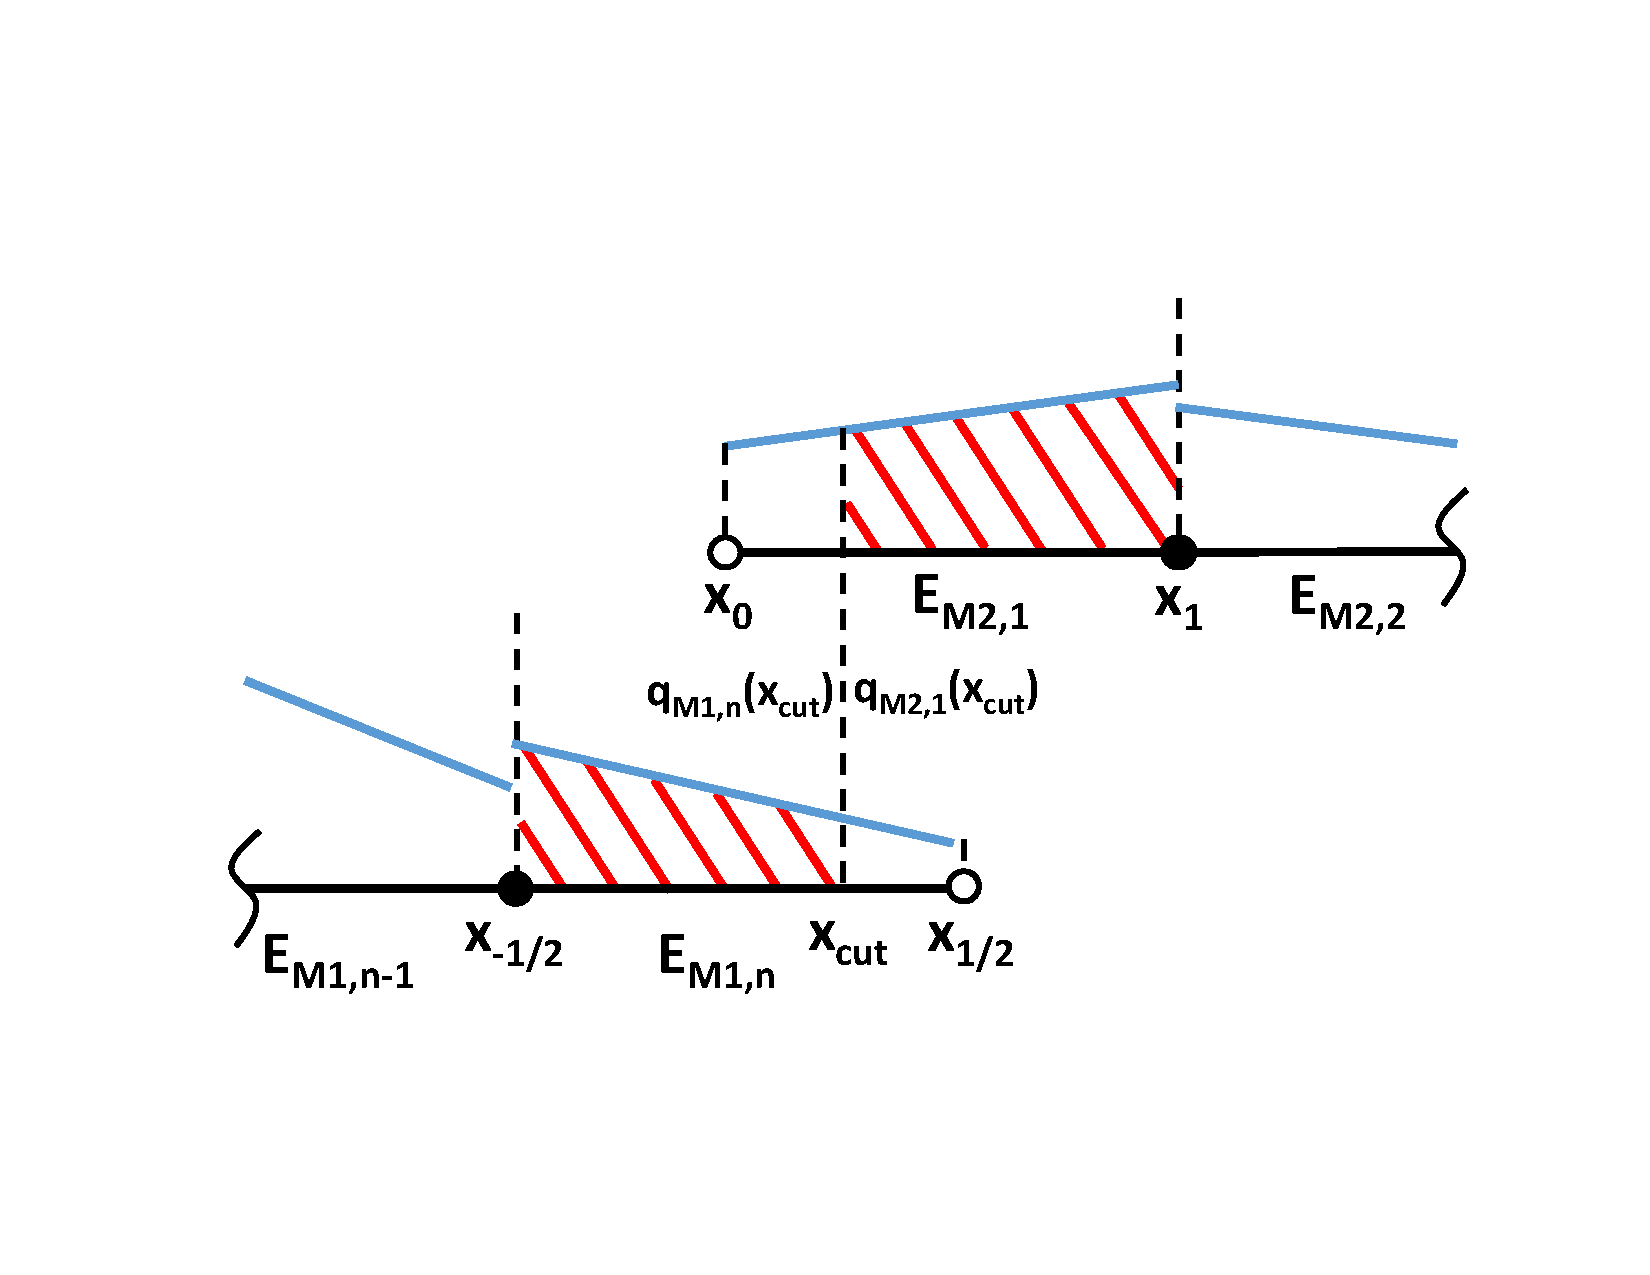
\includegraphics[width=\textwidth,trim={0 4cm 0 4cm},clip]{DGConsOverset.pdf}
  \caption{Schematic describing the conservative overset DG method with two meshes. Portions of the overlap region are removed from each of the volume integrals and the fluxes are calculated at the point where the overlap is split.}
  \label{fig:cons}
\end{figure}

Alternatively, a conservative overset approach is proposed in this work. This approach
is described in Figure \ref{fig:cons}. The overall 
goal of the conservative overset method, is to modify both the volume and flux
integrals of both fringe elements such that they each only account for a portion 
of the overlap region. By doing so, the elements are no longer double counting
the overlap region and are analagous to a single, fully connected grid. 

For the conservative overset approach, both the volume integrals 
and the fluxes will have to be altered. The volume integrals are modified
by subtracting the integral of the cut region, as shown in Equation \eqref{eq:volint}. 

\begin{equation}
\int_a^b f(x) dx = \int_a^c f(x) dx - \int_b^c f(x) dx  \ \ \ \ \text{where} \ a<b<c
\label{eq:volint}
\end{equation}

In this implementation the same number of quadrature points are used to compute
both integrals, maintaining the order of accuracy for the integration. This modification
is done for both the mass matrix and the convective terms. 
The fluxes are handled similarly to the baseline approach however instead of interpolating
the neighboring flux at the end point, now it is interpolated at the point where the overlapping
region is cut, called $x_{cut}$ in Figure \ref{fig:cons}.

Note that how much of the overlap region is cut away from each mesh is up to the user to decide. 
For instance, both meshes can have half of the cut region removed or all of the overlapping
region may be removed from one of the fringe elements while the other 
is left untouched. While any combination of cutting is valid, 
there are implications for numerical stability that will be discussed in the next section. 

\section{Numerical Stability}

While conservative overset method has been shown to lead to a reduction in both L2 and
conservation error (discussed below), integrating over only a portion of the element has been 
observed to make the mass matrix singular and ultimately lead to divergent solutions
under certain circumstances. The stability of the conservative overset method depends on two main
factors: the order of accuracy of the shape functions and the fraction of the element that
is being cut. 

As the spatial order of accuracy is increased, it can be observed that the complete mass matrix
(i.e. over the entire element) becomes larger and more ill-conditioned as a result. This holds
true for both Lagrange (nodal) and Legendre (modal) bases. This is exasperated when 
the mass matrix is computed over only a portion of the element. The more of the element is removed,
the worse the effect is. Because of this, it has been observed that the conservative overset
method fails at high orders (p>5) and when large portions of the elements have been cut away.

To combat this, additional guass points (nshp+3) were added and Tikhonov regularization was added to 
improve the condition of the mass matrix. The regularization essentially solves a similar
L2 minimization problem with a higher condition number (more stable) rather than directly
inverting the mass matrix. While this is a more stable approach, it comes at the cost of additional
bias (and conservation error). The least amount of regularization is added ($\lambda = 0$) in order 
to minimize the added conservation error and retain the benefits from the conservative overset. 
Using the additional gauss points and regularization, the stability was improved to the point that
p=5 simulations with 95\% of the element removed remained stable. However to go beyond p=5 required
so much regularization that the conservation error increased beyond baseline values. 

As an aside, note that by only integrating over a portion of the element, the orthogonality of the
Legendre-based mass matrix is broken. When integrating over a partial element, the mass
matrix is fully populated instead of being purely diagonal, as is the case normally. 

\section{Results}

The advection equation was solved on two meshes on a periodic domain. 
Theoretically, after a single flow through when the wave 
returned to its original position, the solution should 
be identical to the initial condition. Thus the L2 and conservation error were defined as 
shown in Equations \eqref{eq:l2} and \eqref{eq:conserror} below. 

\begin{equation}
e_{L2} = \left ( \int_\Omega (u(x,T) - u(x,0))^2 d\Omega \right )^{1/2}
\label{eq:l2}
\end{equation}

\begin{equation}
e_{cons} = \left | \int_\Omega u(x,0) d\Omega - \int_\Omega u(x,T) d\Omega \right |
\label{eq:conserror}
\end{equation}

\noindent where T is the final time.  The error 
As expected, the L2 error converges at a rate of $(p+1)$. The conservative overset method
shows a lower error than the baseline methods. 

In the test case, the coarse
mesh spanned from [-1,1] and the fine mesh from [-0.268,0.732]. The mesh size of the 
fine grid was half the size of the coarse grid for all cases. A mesh and p-refinement
study was done using both the baseline and conservative overset methods. The timestep
was chosen such that a CFL = 0.01 was achieved. The
results are shown in Figure \ref{fig:error1}. Note that 
these results correspond to the case where half of the overlap region is removed from
each fringe element and Legendre bases are used. The study was repeated for Lagrangian
bases and very little difference was observed.  


\begin{figure}
\centering
  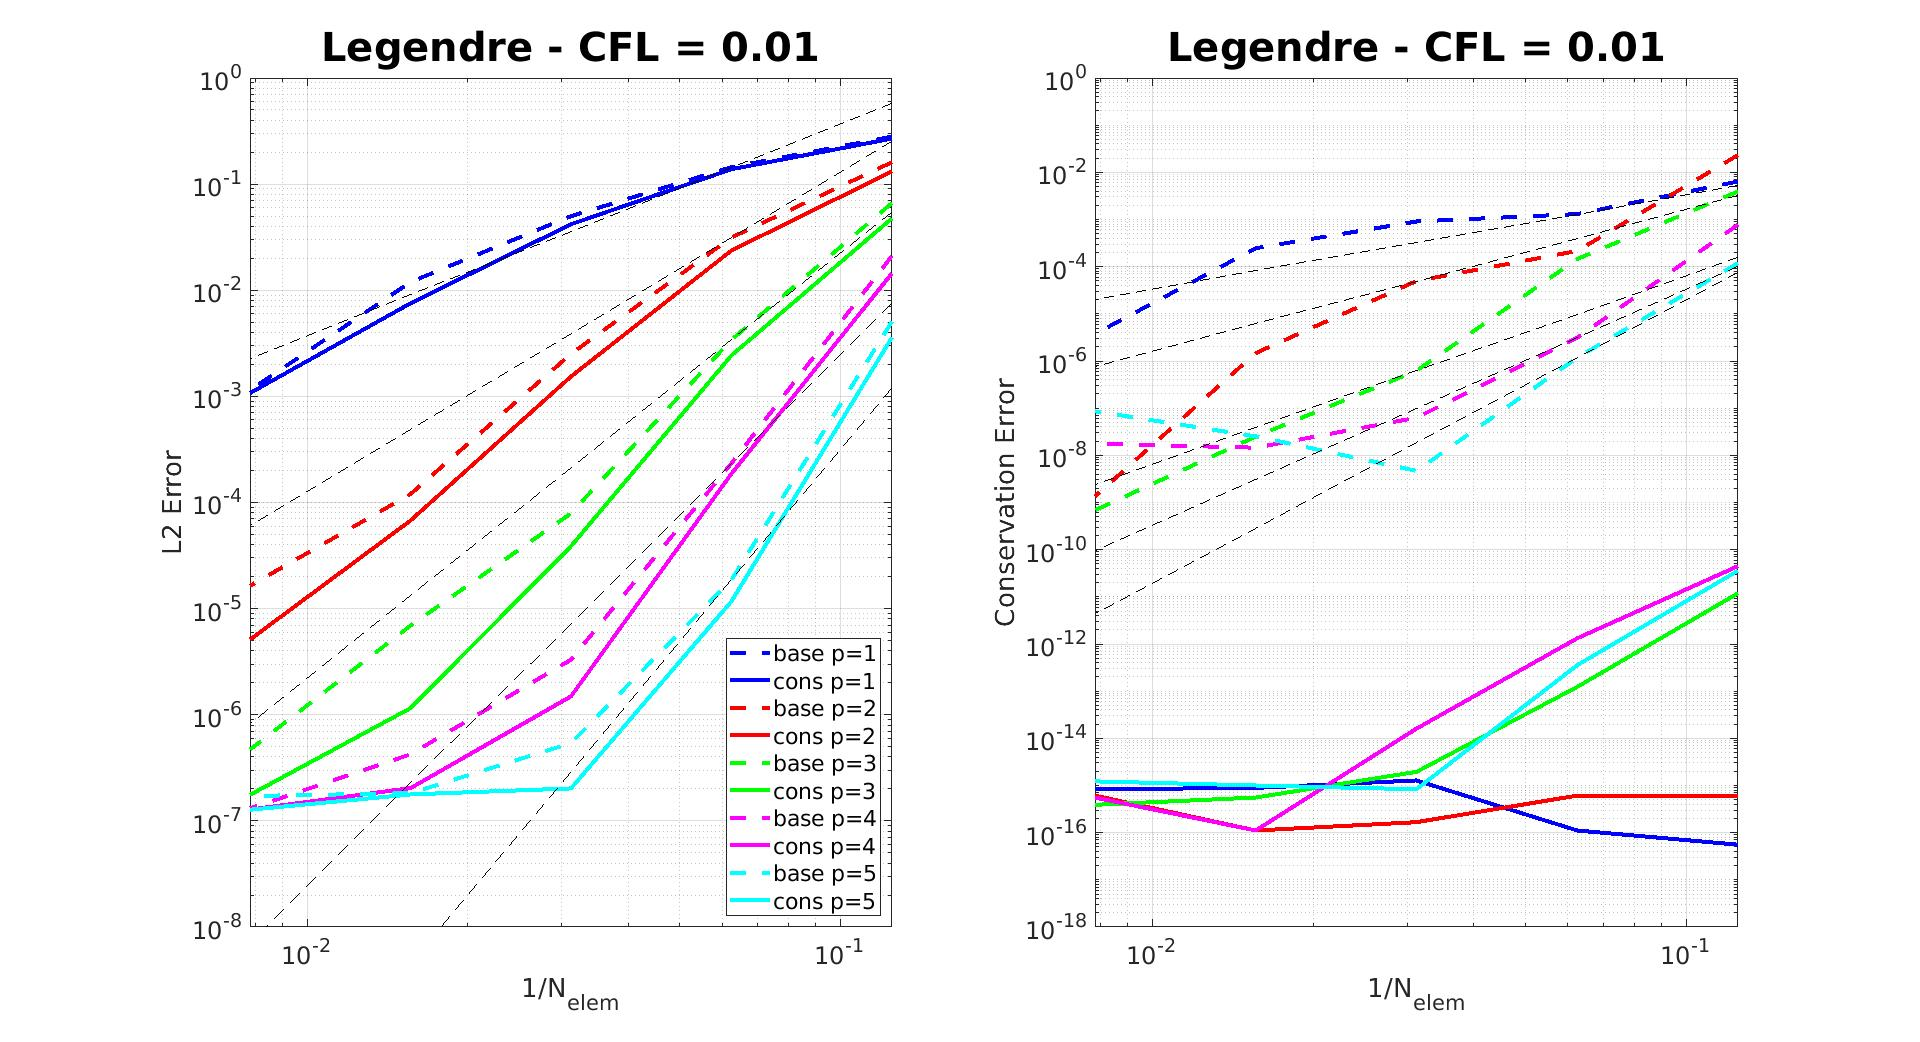
\includegraphics[width=\textwidth]{Convergence_Legendre_CFL0p01.jpg}
  \caption{Convergence plots for L2 and conservation error using the baseline and conservative overset methods}
  \label{fig:error1}
\end{figure}

As can be seen from Figure \ref{fig:error1}, the convergence rate was maintained and 
follows the (p+1) curve for both the baseline and conservative overset methods, although
the conserative method led to consistently lower L2 error. For the conservation error, 
the baseline methods showed non-zero errors that also converged at a rate of (p+1). On
the other hand, the conservative overset errors were consistently at or close to machine epsilon. 
At higher orders with coarse grids, the conservation error using the conservative method was at
its maximum but was still 5 or 6 orders of magnitude smaller than that of the baseline method. 

The effect of the cut fraction was explored. It was found that increasing the cut fraction
makes the cut mass matrix more ill conditioned. As discussed previously, this was addressed
by adding in regularization in the $Ax=b$ matrix solve at the cost of a slight increase
in error. This is shown in Figure \ref{fig:reg} which shows results for 3 cases
where the fine mesh overlaps the coarse mesh by 95\% of the fine mesh length. These 3
cases correspond to 1) the baseline case, 2) conservative overset where 48\% of the coarse element 
was removed (with no regularization), and 3) conservative overset where 95\% of the fine mesh was removed (with
regulariztion). Note that without regularization, the 95\% cut case diverges for p>3 (not shown) but with regularization it is able to 
remain stable until p=5. This additional stability comes at the cost of an increase in the conservation
error but it is still 4+ orders of magnitude lower than the baseline case. The L2 error is unchanged. 

\begin{figure}
\centering
  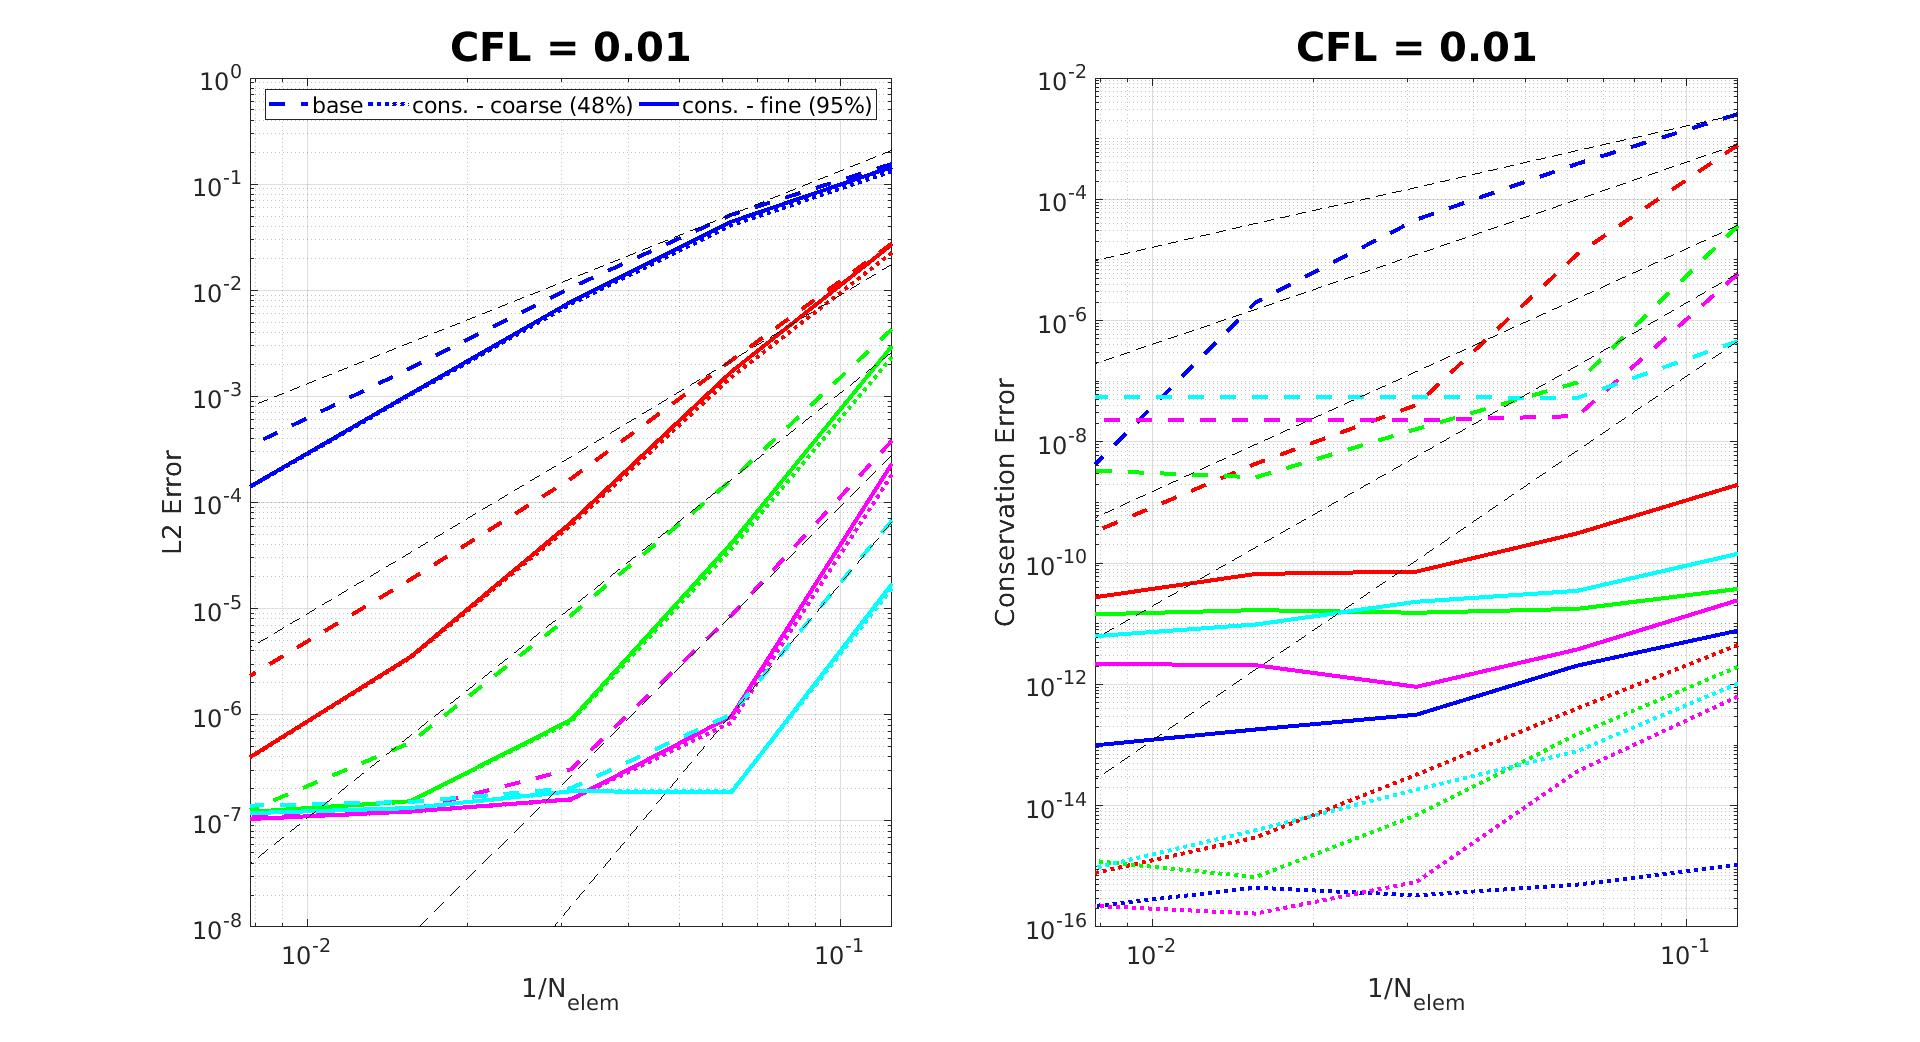
\includegraphics[width=\textwidth]{../src/Convergence_Legendre_CFL0p01_CutLength.jpg}
  \caption{Convergence plots for 1) the baseline case, 2) conservative overset where 48\% of the coarse element was removed, and 3) conservative overset where 95\% of the fine mesh was removed}
  \label{fig:reg}
\end{figure}

Although this method is shown to improve stability, best practice would still be to reduce
the cut length as much as possible by either removing half of the overlap from both
fine and coarse elements or by removing it only from the coarse element. 

\section{Conclusion}
A conservative overset approach is described and applied to a 1D advection problem using
discontinuous Galerkin finite elements. The conservative approach was shown to lead to lower
L2 error as well as eliminating the conservation error. There are some stability issues with 
the approach, although they can be avoided by keeping the spatial order of accuracy below $\approx 6$. 
Regularization was added to improve stability in cases where there is high overlap between
the elements but best practice is still to avoid this situation whenever possible. 

\end{document}
